% Draft Version

\documentclass{beamer}

\usepackage{verbatim} % multilinecomments
\usepackage[utf8]{inputenc}
\usepackage{multicol}

\usetheme{default}


\begin{comment}
\newcommand{\email}[1]
{
    \href{mailto:#1}{#1}
}
\end{comment}

\def \semioturl {\url{http://semiot.ru}}

\title{An implementation of CoAP protocol\\ for Arduino and ESP8266}

% A subtitle is optional and this may be deleted
\subtitle{
    SemIoT project - Semantic technologies for Internet of Things
    \footnote{\semioturl}
}

\author{
    A.~Andreev
    \and
    N.~Klimov
    \and
    D.~Garayzuev
    \and
    I.~Shilin
    \and
    M.~Kolchin
    \and
    D.~Mouromtsev
}
% - Give the names in the same order as the appear in the paper.
% - Use the \inst{?} command only if the authors have different
%   affiliation.


\institute[NRU ITMO] % (optional, but mostly needed)
{
    ITMO University, St.Petersburg, Russia
}



\date{17th FRUCT conference, 2015}
% - Either use conference name or its abbreviation.
% - Not really informative to the audience, more for people (including
%   yourself) who are reading the slides online

\subject{Telecommunications}
    % This is only inserted into the PDF information catalog. Can be left
    % out. 

    % If you have a file called "university-logo-filename.xxx", where xxx
    % is a graphic format that can be processed by latex or pdflatex,
    % resp., then you can add a logo as follows:

    \pgfdeclareimage[height=1cm]{fruct-logo}{fruct_full}
    \pgfdeclareimage[height=1cm]{university-logo}{itmo}
    \pgfdeclareimage[height=1cm]{lab-logo}{logo}
    \titlegraphic{%
        \pgfuseimage{lab-logo}~%
        \pgfuseimage{university-logo}~%
        \pgfuseimage{fruct-logo}%
    }

\begin{document}

    % 1 -- Title
    \begin{frame}
        \titlepage
    \end{frame}

    % 2 -- CoAP
    \begin{frame}
        \begin{center}
            \begin{multicols}{2}
                \huge{\textbf{CoAP://}}\\
                \large{RFC 7252 Constrained Application Protocol}
                \footnote{\url{http://tools.ietf.org/html/rfc7252}}
            \end{multicols}
        \end{center}
        \begin{itemize}
            \item REST model
            \item resources available under a URL
            \item access through GET, PUT, POST, and DELETE methods
            \item working via UDP protocol
        \end{itemize}
    \end{frame}

    % 3 -- MicroCoap
    \begin{frame}
        \begin{multicols}{2}
            
\includegraphics[height=0.5cm,keepaspectratio]{github}
            \huge{\textbf{/microcoap}}\large{\footnote{\url{https://github.com/1248/microcoap}}}\\
            \large{A C implementation that can be compiled for Arduino}
        \end{multicols}
        \begin{itemize}
            \item Implemented CoAP features:
                \begin{itemize}
                    \item CoAP GET, PUT, POST and DELETE methods
                    \item Initial clients support
                    \item Initial endpoints setup
                \end{itemize}
            \item CoAP features required implementation:
                \begin{itemize}
                    \item Resource subscribe option
                    \item Full-fledged CoAP clients support
                    \item Appropriate endpoints setup
                \end{itemize}
        \end{itemize}
    \end{frame}
    
    % 4 -- Prototype
    \begin{frame}
        \begin{center}
        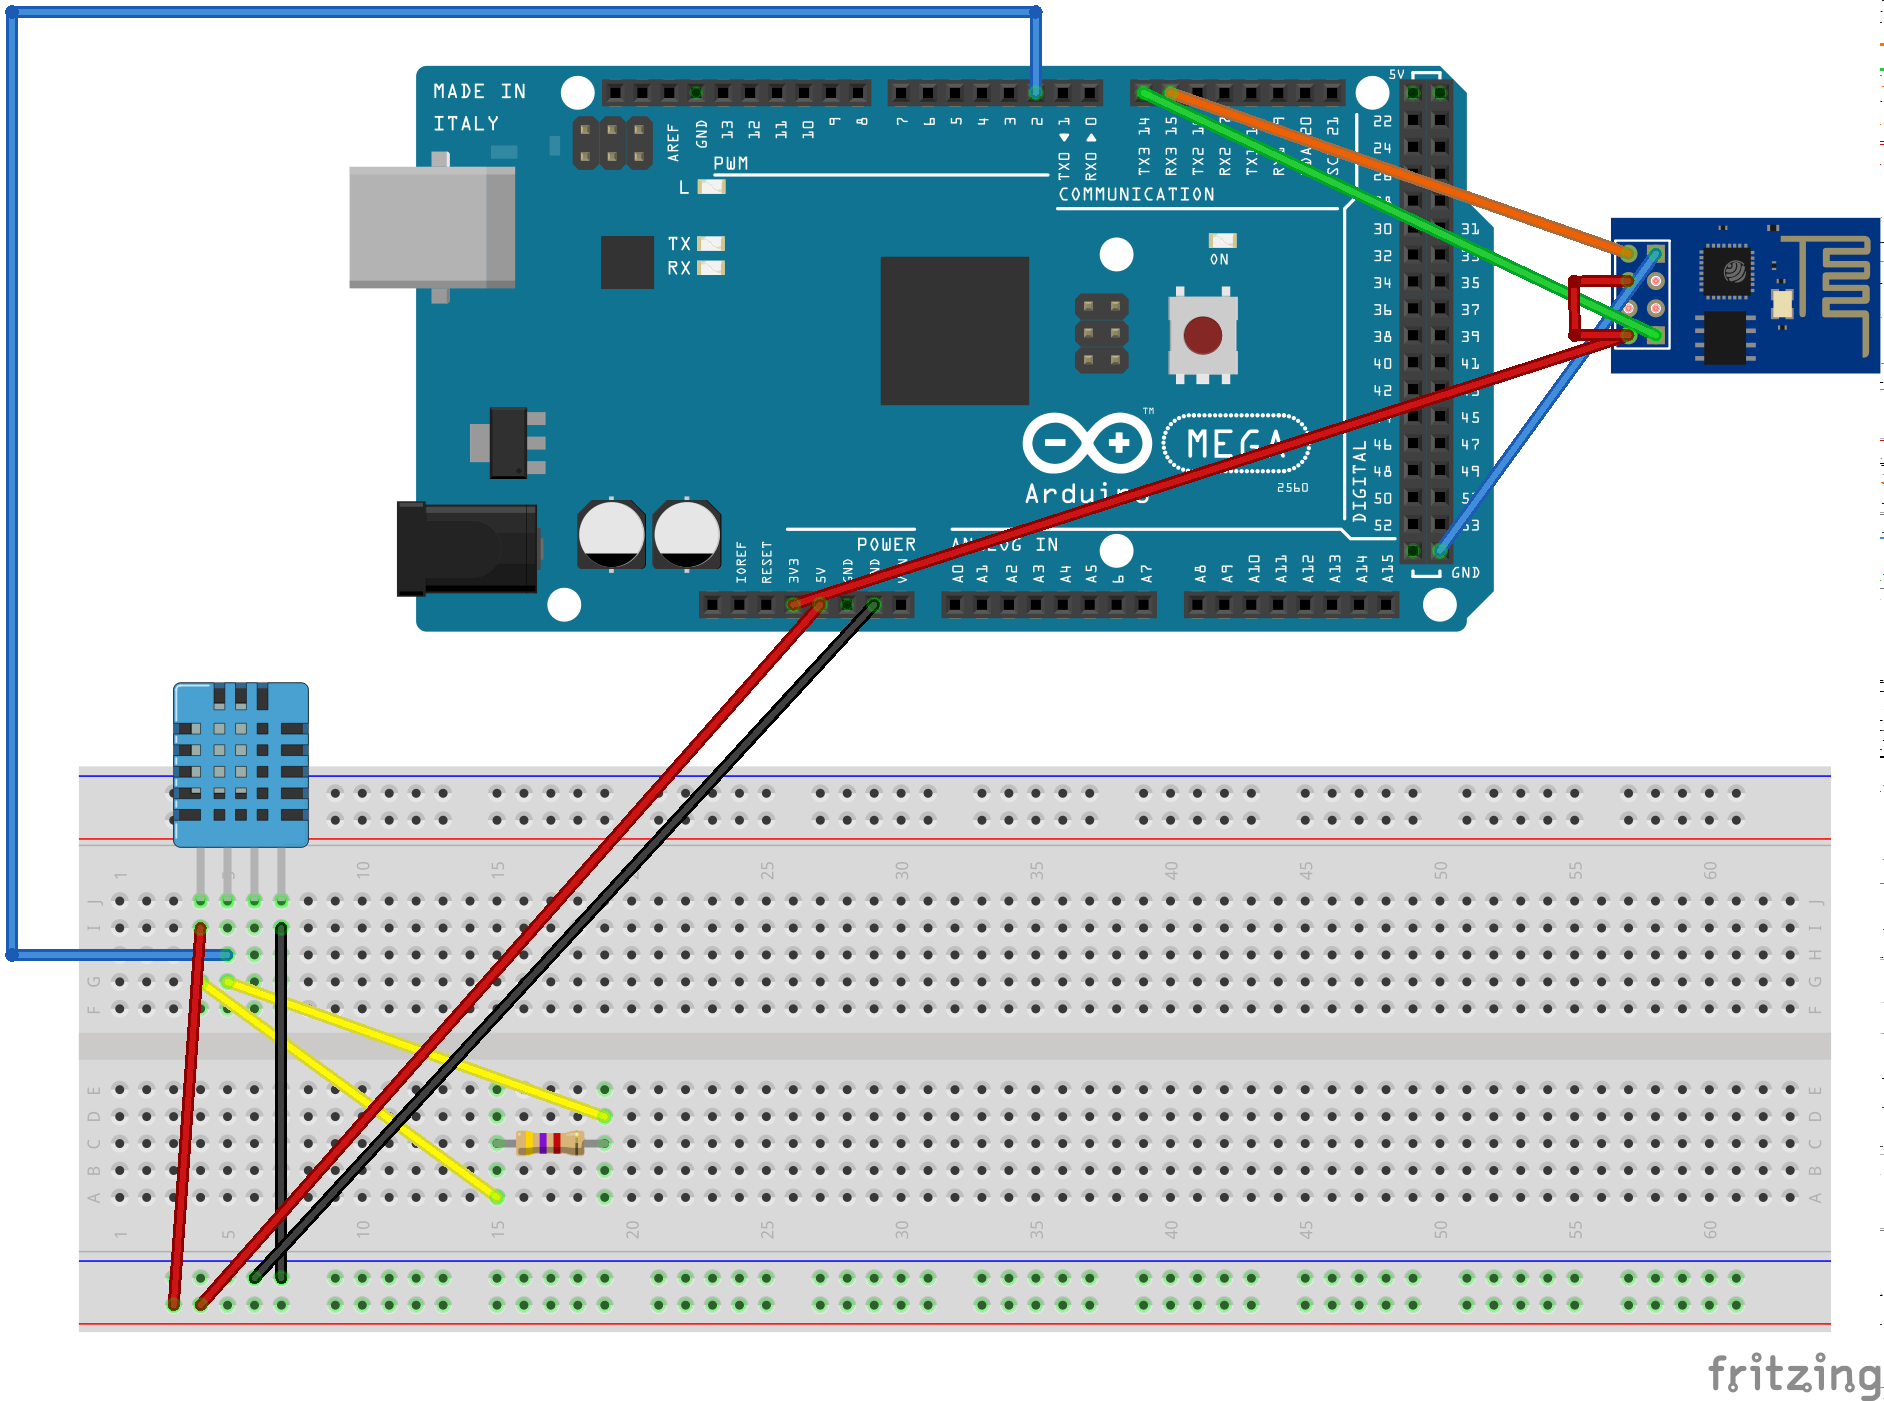
\includegraphics[width=0.7\textwidth,keepaspectratio]{maket}\\
        \textbf{Arduino MEGA2560} with
        \textbf{ESP8266} WiFi-Module
        \footnote{\url{https://github.com/itead/ITEADLIB_Arduino_WeeESP8266}}
        and \\
        \textbf{DHT11} temperature and humidity sensor
        \footnote{\url{https://github.com/niesteszeck/idDHT11}}
        \end{center}
        
    \end{frame}

    % 5 -- Future Plans
    \begin{frame}
        \center\textbf{Future Plans}: wireless device configurations tools\\(mobile application).\\
        \center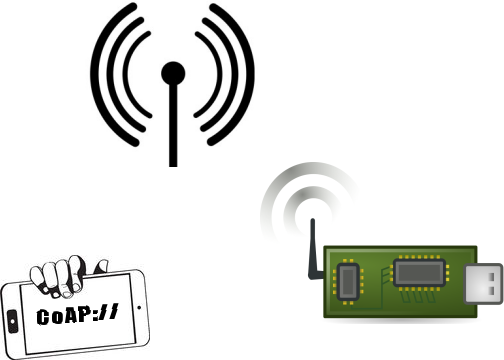
\includegraphics[height=4cm,keepaspectratio]{configuratorapp}\\
    \end{frame}

    % 6 -- SemIoT project
    \begin{frame}
        \begin{center}
            \huge{\textbf{SemIoT} project}\\
            
\includegraphics[height=3cm,keepaspectratio]{Semantic-Web-Logo-by-W3C}
            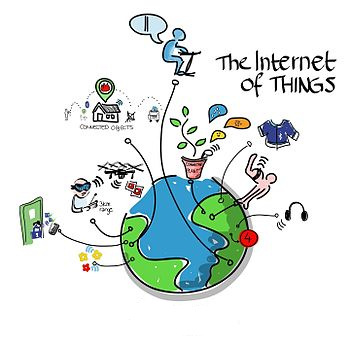
\includegraphics[height=3cm,keepaspectratio]{iot}\\
            Semantic technologies\\
            for Internet of Things
        \end{center}
        \small\center{This work was financially supported by\\
        Ministry of Education and Science of Russian Federation,\\
        Grant \#RFMEFI57514X0101.}
        
    \end{frame}

\end{document}
